\documentclass[a4paper]{article}
\usepackage{listings}
    \lstset{language=Python}
    \lstset{frame=lines}
\usepackage{graphicx}
\usepackage{hyperref}
\usepackage{xcolor}
\usepackage[right]{sidecap}
\usepackage[utf8]{inputenc}


\graphicspath{ {./images/} }
\hypersetup{pdfborder=0 0 0}
\hypersetup{urlcolor=cyan}

\begin{document}
    
    \begin{titlepage}
        \begin{center}
            \hspace{0cm}
            \vfill
            
            \Huge
            CT Projekt: Wordle Multiplayer
            
            \vspace{0.3cm}
            
            \Large
            Wordle-clone mit Multiplayer Funktion
            
            \vspace{0.3cm}
            
            \large
            Alexander Klee
            
            \vspace{0.3cm}
            
            19.03.2022 - 03.06.2022
            
            \vspace{0.3cm}
            \href{https://github.com/DarkCypher-37/WordleMultiplayer}{The Github Repo}
            
            \vfill
            \hspace{0cm}
        \end{center}
    \end{titlepage}

    \tableofcontents
    \pagebreak
    
    \section{Projektbeschreibung}
        \subsection{Motivation}
        Die anfängliche Idee war eine KI für das in 2021 Viral gegangene Wortspiel 'Wordle' zu Programmieren. Verschieden YouTuber haben in der Folge des Hypes verschiedenste Anläufe dazu benutzt. Zum Beispiel hat
        \href{https://www.youtube.com/c/3blue1brown}{\textcolor{blue}{'3Blue1Brown'}} 
        einen sehr Mathematischen Anlauf genommen, wahrend
        \href{https://www.youtube.com/c/GamesComputersPlay}{\textcolor{blue}{'GamesComputersPlay'}} 
        ehr einen Anlauf genommen hätte den ich auch genommen hätte (einen Großen Baum für alle möglichen Wörter herzustellen). Beide sind letzten Endes auf ungefähr dasselbe Optimum gekommen, nämlich das Spiel nach durchschnittlich ~3,421 versuchen zu gewinnen.
        \newline
        Dazu kam, dass ein Mitschüler (Phillip Wissler) den Vorschlag gemacht hatte Wordle mit einem Multiplayer zu versehen. Da ich vor nicht allzu langer Zeit einen Guide zu Network Programing empfohlen bekommen habe, war ich gleich noch mehr interessiert. 
        Also, da schon sehr gute Programme zum 'Lösen' von Wordle entwickelt wurden und die Multiplayer Idee aufkam entschied ich mich für den Multiplayer.
        
        
        \subsection{Wordle}
        Wordle ist ein Wortspiel nicht unähnlich zu einem Kreuzworträtsel - Das ziel ist es ein 5 stelliges Wort zu erraten.
        Der User hat insgesamt 6 Chancen das Wort zu erraten indem der User immer ein 5 stelliges Wort eingibt und danach dem User mitgeteilt wird welche der Buchstaben an der korrekten Position sind, sowie welche Buchstaben im Wort vorkommen und welche nicht.
        
        \subsection{Tech-stack}
        Relativ sicher war ich von Anfang an, dass ich Python für das Projekt verwenden möchte, vor allem da das die Programmiersprache ist mit der ich am meisten Erfahrung habe.
        Unsicher war ich Anfangs wie ich die Multiplayer-funktion einbauen möchte, nachdem ich jedoch keine geeignete Python-Bibliothek für ein Peer-to-Peer Netzwerk gefunden hatte kam ich auf die Idee mit dem Python-Modul 'socket' selbst ein Protokoll für ein Peer-to-Peer Wordle-Spiel zu erstellen.
        Für die Gui (falls ich dazu komme) ist der Plan das Python-Modul 'Arcade' zu verwenden, welches ähnlich wie 'PyGame' und andere Grafikbibliotheken ist.
        Verschiedenste andere Python-Bibliotheken, wie zum Beispiel: 'threading', 'select' und 'queue' habe ich verwendet um diverse Probleme zu lösen.
        
    
    \section{Das Programm}
        \subsection{Wordle}
            Bei Wordle muss der Spieler ein 5 stelliges Lösungswort erraten. Dies kann der Spieler bewerkstelligen, indem er ein Wort mit 5 Buchstaben eingibt.
            Der Spieler kann insgesamt 6 mal ein Wort eingeben um das Lösungswort zu erraten. Schafft er es nicht innerhalb dieser 6 versuche, so verliert er das Spiel. 
            Jedoch muss der Spieler das Lösungswort nicht komplett willkürlich aus dem nichts heraus erraten, sondern er bekommt langsam mehr Informationen über das Lösungswort. Sobald der Spieler ein vollstandiges Wort eingibt, wird dem Spieler jeder Buchstabe markiert, bei dem  die Position richtig ist, oder das Lösungswort denselben Buchstaben enthält.
            
            \subsubsection{Der Match Algorithmus}
                Sobald der User ein Wort vollständig eingegeben hat, also 5 Buchstaben, wird gecheckt ob das Wort ein Wort der Englischen Sprache ist und welche Buchstaben zum einen die richtige Position haben, welche Buchstaben zwar nicht die richtige Position haben aber dennoch im Wort vorkommen und welche Buchstaben gar nicht im Lösungswort vorkommen.
                
                Zuerst erstellen wir eine liste mit 5 Einträgen welche 'nicht im Lösungswort Vorkommend' repräsentiert (In Python habe ich dafür das Enum 'CharStatus' kreiert).
                
                Danach wird aus sowohl dem Lösungswort und dem aktuellem Wort das der User eingegeben hat alle Buchstaben die an der richtigen Position sind raus gefiltert und dementsprechend in der Liste an dem Index des Buchstabens der Wert auf CharStatus.correct\_position gesetzt.
                
                Im zweiten Durchlauf über das Wort, welches der User eingegeben hat, wird geschaut ob die einzelnen Buchstaben im Lösungswort vorkommen. Dabei wird nach first-match-wins principle gearbeitet, sodass wenn der User-guess mehr als ein 'a' enthält und das Lösungswort nur ein 'a' enthält, wird nur das erste 'a' als CharStatus.word\_contains markiert, das zweite 'a' wird als CharStatus.word\_doesnt\_contain in der Liste gespeichert.
                
                \begin{figure}[t]
                    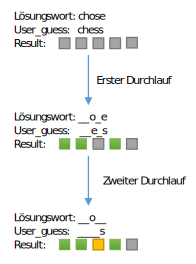
\includegraphics{images/WordleAlgo.png}
                    \centering
                    \caption{Beispiel ablauf des Wordle-Match-Algorithmus}
                \end{figure}
                
            \pagebreak
            \subsubsection{Multiplayer}
                Im Multiplayer geht es nicht nur darum das Wort zu erraten, sondern dazu auch noch schneller zu sein als seine Mitspieler.
                Jedem Spieler wird jetzt nicht nur sein eigener Fortschritt angezeigt, sondern bekommt noch zusätzlich den Fortschritt der Mitspieler zu sehen. Natürlich ohne anzuzeigen welche tatsächlichen Worter die Mitspieler eingegeben haben, sonst könnte der Spieler einfach abschreiben. Stattdessen wirden nur die farbigen Boxen angezeigt, sodass ein Spieler sieht wie weit seine Mitspieler schon sind.
                Leider ist zu diesem Zeitpunkt nur ein Mehrspieler Spiel mit 2 Personen möglich, da die Sockets nicht vollständig geschlossen werden.
                
            
        
        \subsection{die GUI}
            Sobald der User das Spiel startet öffnet sich die GUI. Dort kann der User auswählen, ob er einem Netzwerk von jemand anderem beitreten möchte oder ob er ein neues Netzwerk erstellen möchte. 
            Sobald 'Create Network' ausgewählt wurde, muss der User nur noch den Usernamen eingeben und dann wird eine Game-Instanz erstellt und das Spiel gestartet. 
            Wenn 'Join Network' ausgewählt wurde, wird der User vorher noch nach dem Port und der IP-Adresse, sowie dem Gamekey gefragt und dann sich zu dem jeweiligem Netzwerk verbunden.
            Das ganze ist geregelt über arcade.View Instanzen, das heißt gibt eine Window-Instanz, welche ein arcade.View Objekt hat, in welchem 60-mal pro Sekunde die Funktionen on\_draw() und on\_update() aufgerufen wird.
            
            Während des Spieles ist die View 'GameView' aktiv. 
            
            In der Datei Shapes.py sind verschiedenste Klassen um das Zeichnen von zum Beispiel Buttons oder Textlables einfacher zu machen.
            Ebenfalls ist dort eine Klasse mit dem Namen WordTable, mit welchem die Tabelle für den Spielstand während des Spieles Angezeigt wird.
            Diese Objekte haben eine einfache draw()-funktion, welche einfach in der on\_draw() Methode des Fenster Objektes (bzw. der View-Instanz) aufgerufen werden kann um das jeweilige Element auf den Bildschirm zu Zeichnen.
            
        
        \subsection{Networking}
            
            \subsubsection{TCP / IP}
                Jeder PC der ans Internet angeschlossen ist, also so gut wie jeder PC hat eine IP-Adresse. Mit Hilfe dieser IP-Adresse kann man von jedem PC zu jedem anderen PC Nachrichten mit TCP senden. Dabei kann man sich vorstellen, dass IP wie Haus-Adressen funktionieren und TCP der Briefträger, wobei das nicht ganz richtig wäre denn TCP versendet keine Nachrichten, sondern garantiert einen kontinuierlichen und fehlerfreien bytesstream, also kommen die Einsen und Nullen nacheinander an wie auf einem Förderband. 
                
                Damit nicht jedes Haus nur ein Förderband haben kann, hat man Ports eingeführt, zu vergleichen mit verschiedenen Haustüren ins selbe Haus, wofür ein Förderband immer eine Haustüre brauch.
                
                Am Ziel angekommen werden sie zuerst in einem Buffer zwischen Gespeichert, 
                welcher dann mit socket.recv(Anzahl\_der\_Bytes) ausgelesen werden kann. (In der Briefträger Analogie wäre dies dann Wahrscheinlich der Briefkasten, allerdings habe ich diesen Vergleich schon viel zu weit gestreckt)
                
                Da IPv4 eine 32-Bit Zahl ist gab es nur $2^{32} = 4294967296$ IP-Adressen, also gerade mal 4 Milliarden IP-Adressen, was nicht einmal annähernd genug wäre wenn jede Person auf der Welt nur einen Computer besitzen dürfte. (Vor allem nicht wenn man gut die Hälfte aller IP-Adressen an private Firmen verschenkt) Aus diesem Grund wurden Private und Public IP-Adressen eingeführt. Welche ungefähr so funktionieren: jeder Haushalt bekommt eine Public IP-Adresse, mit welchem die Außenwelt mit dem in dem Haushalt stehenden Router kommuniziert. Dieser Router teilt jedem Endgerät (Handy, PC, usw.) eine Private IP-Adresse zu, welche nur innerhalb des Haushalt-Netzwerkes funktioniert. Möchte jetzt mein Handy mit einem Server in den Weiten des Internets reden, muss das Handy zunächst die Nachricht mithilfe der Privaten IP-Adresse dem Router zuschicken, welcher dann mit der Public IP-Adresse dem Server die Nachricht zuschicken kann.
                
                Soweit so gut, das Problem für mein Projekt hierbei ist, dass nicht nur diverse Firewalls im Weg meines Programms stehen, sondern ich auch noch 'NAT hole punching' (den Router dazu überzeugen, meine Nachrichten mithilfe seiner Public IP weiterzuleiten) benötigen wurde um zwei zufällige PCs auf der Welt zum zusammen zum Wordle spielen bringen zu können.
                
                Um keinerlei Probleme mit Firewalls oder mit unheimlich und zufällig verschwindenden Pakete zu haben bietet es sich an den 'localhost' zu nutzen, auch genannt 'loopback', befindet sich dieser an der IP-Adresse '127.x.x.x'. Diese Adresse lässt die Pakete nie vom Computer los, sondern leitet die Pakete wieder in sein eigenes Postfach (diese Analogie schon wieder... ).
                
                Heutzutage ist geplant von IPv4, sowie Private und Public IP-Adressen zu einem neueren Standard 'IPv6' zu wechseln, welcher 128 Bits hat, jedoch ist allgemeine Adaption des Standards nur schleichend am vorankriechen.
                
                
                \begin{figure}[t]
                    \includegraphics[width=12cm]{images/public_private_networks.jpg}
                    \centering
                    \caption{Private und Public-IP-Adressen wurden eingeführt, sodass nicht jedes Endgerät eine eigene IP-Adresse braucht}
                \end{figure}
            
            \pagebreak
            \subsubsection{das Worlde-Protokoll (WTP)}
                Der Großteil meines Projektes war es das WTP (Wordle-Transfer-Protokoll) zu definieren und zu implementieren.
                Das WTP besteht aus verschiedenen Nachrichten, welche von nur 25 Bytes bis zu 4121 Bytes groß sein können. Die ersten 25 Bytes sind immer der Header, die Folgenden 0 bis $2^{14} = 4096$ Bytes sind die 'message', welche im gegensatz zum Header für jeden verschiedenen Message-Typ unterschiedlich sein kann. \\
            
                \vspace{10px}
                
                \noindent\makebox[\textwidth]{%
                \begin{tabular}{c|c|c|c|c|c}
                    \multicolumn{5}{c|}{Header} & Message\\
                    \hline \hline
                    4bytes & 4bytes & 8bytes & 8bytes & 1byte & 0 .. 4096bytes\\
                    \hline
                    Magic Number & Size & Gamkey Sender & Identifier & Message Type & Message String
                \end{tabular}
                }
                
                \vspace{20px}
                
                \begin{itemize}
                    \item Die 'Magic Number' ist immer genau 0x8b0968b3 und wird benutzt um überprüfen ob die nachrichten noch synchron ankommen (also dass nicht wenn versucht wird die 'Size' zu nutzen aus versehen ein anderer Teil der Nachricht gelesen wird).
                    \item Die 'Size' bestimmt die länge des variablen Teil der Message (genannt Message String)
                    \item Der 'Gamekey' wird genutzt, ungefähr wie ein Passwort, um zu überprüfen ob der sender der Message tatsächlich auch erlaubt sein sollte mit dem spiel zu interagieren.
                    \item Der 'Sender Identifier' wird genutzt um zu bestimmen, welcher Spieler das Paket gesendet hat.
                    \item Die 'Message Type' wird genutzt um zu bestimmen, wie der Empfänger auf die Message reagieren soll und wie dieser den 'Message String' zu Interpretieren hat.
                    \item Der 'Message String' wird genutzt um verschiedenste Informationen zu übertragen, zum Beispiel welche Buchstaben ein Spieler zuletzt hinzugefügt hat, oder den Usernamen des Spielers.
                \end{itemize}
                
                
                \noindent\makebox[\textwidth]{%
                    \begin{tabular}{ c|c|p{6cm}|p{2cm} }
                        Message Type Char & Message Type & Beschreibung & Message String\\
                        \hline \hline
                        j & join request & ein neuer Spieler möchte dem Netzwerk beitreten & Port, Username\\
                        \hline
                        k & join response accept & bestätigung des Beitrittes eines neuen Spielers & identifier für den neuen Spieler, Lösungswort\\
                        \hline
                        m & join response deny & ablehnung des Beitrittes eines neuen Spielers & Grund \\
                        \hline
                        n & join note & benachrichtige einen Spieler, dass der Sender der Nachricht erfolgreich dem Netzwerk beigetreten ist & Username\\
                        \hline
                        o & join note response & Antwort auf eine join note & username \\
                        \hline
                        s & start game & benachrichtigt andere Spieler, davon dass der Sender nun beginnt zu Spielern & Unicode Timestamp \\
                        \hline
                        e & error info & Zur Thread-sicheren error weiterleitung vom NetworkCommunicator zum NetworkHandler & error message \\
                        \hline
                        r & ready & benachrichtigt andere Spieler davon dass der Sender bereit zum Spielen ist & - \\
                        \hline
                        u & unready & benachrichtigt andere Spieler davon dass der Sender nicht mehr bereit zum Spielen ist & - \\
                        \hline
                        c & char add & benachrichtigt andere Spieler davon dass der Sender ein Buchstaben zum WordTable hinzugefügt hat & Buchstabe \\
                        \hline
                        d & remove char & benachrichtigt andere Spieler davon dass der Sender ein Buchstaben vom WordTable entfernt hat & Buchstabe \\
                        \hline
                        w & word & benachrichtigt andere Spieler davon dass der Sender ein Wort zum WordTable hinzugefügt hat & Wort\\
                        \hline
                        l & leave & benachrichtigt andere Spieler davon dass der Sender das Netzwerk verlässt & - \\
                    \end{tabular}
                }
                
                
            \pagebreak
            \subsubsection{threading und queues}
                Das Senden und Empfangen wird im NetworkCommunicator gemacht, der NetworkHandler stellt die Nachrichten zusammen und stellt diese in eine FiFo - queue, sodass der NetworkCommunicator die Messages dann Aberbeiten kann.
                
                Eine FiFo-Queue ist sich sehr ähnlich einer Warteschlange beim Bäcker vorzustellen, die Person, die als erstes in der Schlange kam, wird auch als erstes abgearbeitet
            
                \begin{figure}[t]
                    \includegraphics[width=7cm]{images/FiFoQueue.png}
                    \centering
                    \caption{Verhalten einer FiFo-Queue}
                \end{figure}
            
                Für das Programm heißt das, dass die Nachrichten, welche von dem NetworkHandler in die Warteschlange gepackt wurden werden nach und nach in der selben Reihenfolge von dem NetworkCommunicator, welcher in einem separaten Thread sitzt gesendet.
                Der ganze Aufwand, weshalb Warteschlangen verwendet werden ist nämlich genau dem geschuldet: Dass der NetworkCommunicator in einem separaten Thread sitzt. Das ganze hat nämlich zu Folge, dass eine sogenannte 'Race condition' entstehen kann, was in Kurzform bedeutet, dass eine variable, welche von einem Thread gelesen wird gleichzeitig von einem anderen Thread bearbeitet, sodass der erste Thread nun den falschen 'Eindruck' von der Variable bekommen hat.
                Um das zu vermeiden nutzt man sogenannte 'mutexes' (MUTual EXclusions), welche genau das verhindern, indem immer nur ein einzelner Thread auf dieselbe Variable zugreifen kann.
                \footnote{'race condition's sind in Python sehr selten und man muss diese praktisch mit absicht hervor rufen}
                \footnote{Mutexes müssen ein paar sehr interessante assembly operationen durchführen (atomic operations), welche zum Beispiel gleichzeitig ein Wert austauschen während sie im selben Maschinen Zyklus noch testen ob sie das 'lock' vom Mutex besitzen, \href{https://www.youtube.com/watch?v=1tZhmTnk-vc}{\textcolor{blue}{Mehr info hier}}}
                
                Verschiedene Threads müssen genutzt werden, da viele verschiedene Funktionen im Umgang mit Sockets einige Zeit brauchen, bis diese fertig sind und die Gui sollte in der selben Zeit trotzdem noch auf User input reagieren.
            
            \subsubsection{Senden und Empfangen}
                Um das senden und empfangen mit Sockets Kurz zu fassen: Nachdem der main\_socket erstellt wurde, wird durchgehend mit select.select() nachgeschaut, ob es neue Verbindungen gibt, auf denen das Programm lesen oder schreiben kann. \footnote{lesen und schreiben daher, da für moderne Betriebsysteme praktisch alles ein File ist, auch eine Internetverbindung wird über sogenannte 'file descriptors' gemanaged, genau wie eine normale Datei} \footnote{offene Verbindungen sind immer schreib-bar, weshalb wir nur dann Sockets in den schreib-Parameter für select.select() übergeben, wenn wir auch etwas haben, das wir senden wollen} Sollte kein socket zum schreiben oder lesen bereit sein, timed select() nach einer Sekunde aus um zu überprüfen, ob der NetworkHandler neue Messages zum senden in die FiFo-Queue geschoben hat.
                Sollte es zu Lesende Sockets geben, empfangen wir darauf die gesendeten Messages und schließen den Socket.
                Sollte es Sockets geben in welche das Programm schreiben kann, werden die passenden Nachrichten gesendet und der Socket geschlossen. \footnote{genau hier beim schließen des Sockets tritt ein Bug auf der es verhindert, dass mehr als 2 Personen miteinander spielen können. Der Rest des Programmes könnte theoretisch unendlich viele Mitspieler bearbeiten}
                
                Findet der NetworkCommunicator eine neue Message in der Queue, fängt dieser an sie zu bytes zu verwandeln, mit Hilfe des Python-Modules 'struct', kann man C-identische Structs 'packen', welche sich als Bytes einfach versenden lassen.
                Wichtig ist hierbei zu beachten, dass bei Datentypen, welche Länger als Ein byte sind verschiedene Hersteller die Datentypen verkehrt herum speichern. Allgemein wurde sich darauf geeinigt jede ausgehende nachrichten mit Network-byte-order zu versehen, öfters Big-Endian genannt.
                
                Wenn der NetworkCommunicator merkt, dass eine 'l'-Message (also eine leave-Message) gesendet wird, fängt dieser an alle Verbindungen 'sanft' bzw. 'sauber' zu schließen, sodass das Programm Problemlos beendet werden kann. 
            
        \subsection{UML}
            Die Verhältnisse der Klassen waren deutlich zu Groß um sie hier einzufügen, es sind jedoch im Ordner Bilder Vorhanden
            \begin{figure}[h]
                \includegraphics[width=7cm]{images/Files.png}
                \centering
                \caption{Die Verhältnisse der Files}
            \end{figure}
        
    \pagebreak
    
    \section{Quellen}
        \begin{itemize}
            \item https://beej.us/guide/bgnet/html/
            \item http://stupidpythonideas.blogspot.com/2013/05/sockets-are-byte-streams-not-message.html
            \item https://docs.python.org/3/library/struct.html
            \item https://docs.python.org/3/library/select.html
            \item https://docs.python.org/3/library/queue.html
            \item https://docs.python.org/3/library/socket.html
            \item https://docs.python.org/3/library/threading.html
            \item https://steelkiwi.com/blog/working-tcp-sockets/
            \item https://realpython.com/python-sockets/
            \item https://docs.microsoft.com/en-us/windows/win32/winsock/windows-sockets-error-codes-2
            \item https://docs.microsoft.com/en-us/windows/win32/winsock/windows-sockets-error-codes-2
            \item https://stackoverflow.com/questions/58468858/python-socket-issues-oserror-errno-10035
            \item https://realpython.com/intro-to-python-threading/#threading-objects
        \end{itemize}
    \include{name}
    
\end{document}